% !TEX TS-program = lualatex
% !TEX encoding = UTF-8 Unicode
\documentclass[12pt,a4paper]{article}

\IfFileExists{src/libs/body.tex}{% --- body.tex ---
\usepackage{pdfpages}
\usepackage{fontspec}
% Prefer Times New Roman when available; fall back in container environments.
\IfFontExistsTF{Times New Roman}{
  \setmainfont{Times New Roman}
}{
  \setmainfont{Liberation Serif}
}
\usepackage[vietnamese]{babel}

% Page layout and spacing
\usepackage[left=3cm,right=2cm,top=2cm,bottom=2cm]{geometry}
\usepackage{titlesec}
\usepackage{setspace}

% Silence noisy warnings
\usepackage{silence}
\WarningFilter{transparent}{Loading aborted}
\WarningFilter{hyperref}{The anchor of a bookmark and its parent's}

% Core packages
\usepackage{float}
\usepackage{svg}
\usepackage{graphicx}
\graphicspath{{assets/}{../assets/}{../../assets/}}
\svgpath{{assets/}{../assets/}{../../assets/}}
\usepackage{enumitem}
\usepackage{array}
\usepackage{tabularx}
\usepackage{multirow}
\usepackage[table]{xcolor}
\usepackage{ulem}
\usepackage{xurl}

% ====== THÊM 2 GÓI NÀY ĐỂ FIX LỖI ADJUSTBOX VÀ FOREST ======
\usepackage{adjustbox}
\usepackage[edges]{forest}
% ============================================================

% TikZ
\usepackage{tikz}

% ====== BỔ SUNG FIT, BACKGROUNDS, TREES VÀO DANH SÁCH ======
\usetikzlibrary{calc, arrows.meta, shapes.geometric, positioning, fit, backgrounds, trees}

% Table tuning
\renewcommand{\tabularxcolumn}[1]{m{#1}}
\hbadness=10000
\hfuzz=10000pt

% Shared commands
\newcommand{\subsecheading}[1]{%
    \par\vspace{2pt}%
    \hspace{1.5em}\textbf{#1}%
    \par\vspace{2pt}%
}
\newcommand{\introtext}[1]{%
    \par\hspace{3.0em}#1\par%
}
\newcommand{\StandaloneDocumentSetup}[2]{%
  \pagenumbering{arabic}%
  \ApplyStandardFooter{#1}{#2}%
}
\newcommand{\StandaloneSectionSetup}[2]{%
  \ApplyStandardFooter{#1}{#2}%
}

% Math
\usepackage{amsmath}

% Hyperref
\usepackage{hyperref}
\hypersetup{
    colorlinks=true,
    linkcolor=black,
    filecolor=magenta,
    urlcolor=blue,
}}{% --- body.tex ---
\usepackage{pdfpages}
\usepackage{fontspec}
% Prefer Times New Roman when available; fall back in container environments.
\IfFontExistsTF{Times New Roman}{
  \setmainfont{Times New Roman}
}{
  \setmainfont{Liberation Serif}
}
\usepackage[vietnamese]{babel}

% Page layout and spacing
\usepackage[left=3cm,right=2cm,top=2cm,bottom=2cm]{geometry}
\usepackage{titlesec}
\usepackage{setspace}

% Silence noisy warnings
\usepackage{silence}
\WarningFilter{transparent}{Loading aborted}
\WarningFilter{hyperref}{The anchor of a bookmark and its parent's}

% Core packages
\usepackage{float}
\usepackage{svg}
\usepackage{graphicx}
\graphicspath{{assets/}{../assets/}{../../assets/}}
\svgpath{{assets/}{../assets/}{../../assets/}}
\usepackage{enumitem}
\usepackage{array}
\usepackage{tabularx}
\usepackage{multirow}
\usepackage[table]{xcolor}
\usepackage{ulem}
\usepackage{xurl}

% ====== THÊM 2 GÓI NÀY ĐỂ FIX LỖI ADJUSTBOX VÀ FOREST ======
\usepackage{adjustbox}
\usepackage[edges]{forest}
% ============================================================

% TikZ
\usepackage{tikz}

% ====== BỔ SUNG FIT, BACKGROUNDS, TREES VÀO DANH SÁCH ======
\usetikzlibrary{calc, arrows.meta, shapes.geometric, positioning, fit, backgrounds, trees}

% Table tuning
\renewcommand{\tabularxcolumn}[1]{m{#1}}
\hbadness=10000
\hfuzz=10000pt

% Shared commands
\newcommand{\subsecheading}[1]{%
    \par\vspace{2pt}%
    \hspace{1.5em}\textbf{#1}%
    \par\vspace{2pt}%
}
\newcommand{\introtext}[1]{%
    \par\hspace{3.0em}#1\par%
}
\newcommand{\StandaloneDocumentSetup}[2]{%
  \pagenumbering{arabic}%
  \ApplyStandardFooter{#1}{#2}%
}
\newcommand{\StandaloneSectionSetup}[2]{%
  \ApplyStandardFooter{#1}{#2}%
}

% Math
\usepackage{amsmath}

% Hyperref
\usepackage{hyperref}
\hypersetup{
    colorlinks=true,
    linkcolor=black,
    filecolor=magenta,
    urlcolor=blue,
}}
\IfFileExists{src/libs/header.tex}{% --- header.tex ---
\usepackage{fancyhdr}
\setlength{\headheight}{15.5pt} % Thêm dòng này để fix cảnh báo chiều cao
%\setlength{\headheight}{14.5pt}
\addtolength{\topmargin}{-2.5pt}

\pagestyle{fancy}
\fancyhf{}
\renewcommand{\headrulewidth}{0pt}
\renewcommand{\footrulewidth}{0pt}

\newcommand{\ApplyStandardHeader}{%
  \fancyhead[L]{%
    \begin{minipage}[t]{0.795\linewidth}%
      UIT \textbar{} SS004.F21 \textbar{} Nhóm 03 \textbar{} Đồ án cuối kỳ%
    \end{minipage}%
    \vrule%
    \begin{minipage}[t]{0.185\linewidth}%
      \centering cTetris%
    \end{minipage}%
  }%
}

\ApplyStandardHeader
}{% --- header.tex ---
\usepackage{fancyhdr}
\setlength{\headheight}{15.5pt} % Thêm dòng này để fix cảnh báo chiều cao
%\setlength{\headheight}{14.5pt}
\addtolength{\topmargin}{-2.5pt}

\pagestyle{fancy}
\fancyhf{}
\renewcommand{\headrulewidth}{0pt}
\renewcommand{\footrulewidth}{0pt}

\newcommand{\ApplyStandardHeader}{%
  \fancyhead[L]{%
    \begin{minipage}[t]{0.795\linewidth}%
      UIT \textbar{} SS004.F21 \textbar{} Nhóm 03 \textbar{} Đồ án cuối kỳ%
    \end{minipage}%
    \vrule%
    \begin{minipage}[t]{0.185\linewidth}%
      \centering cTetris%
    \end{minipage}%
  }%
}

\ApplyStandardHeader
}
\IfFileExists{src/libs/footer.tex}{% --- footer.tex ---
\usepackage{lastpage}

\newcommand{\ApplyStandardFooter}[2]{%
  \fancyfoot[L]{%
    \begin{minipage}[t]{0.795\linewidth}%
      Document ID: #1%
    \end{minipage}%
    \vrule%
    \begin{minipage}[t]{0.185\linewidth}%
      \centering\thepage/\pageref{#2}%
    \end{minipage}%
  }%
  \fancypagestyle{plain}{%
    \fancyhf{}%
    \renewcommand{\headrulewidth}{0pt}%
    \renewcommand{\footrulewidth}{0pt}%
    \ApplyStandardHeader%
    \fancyfoot[L]{%
      \begin{minipage}[t]{0.795\linewidth}%
        Document ID: #1%
      \end{minipage}%
      \vrule%
      \begin{minipage}[t]{0.185\linewidth}%
        \centering\thepage/\pageref{#2}%
      \end{minipage}%
    }%
  }%
  \pagestyle{fancy}%
}
}{% --- footer.tex ---
\usepackage{lastpage}

\newcommand{\ApplyStandardFooter}[2]{%
  \fancyfoot[L]{%
    \begin{minipage}[t]{0.795\linewidth}%
      Document ID: #1%
    \end{minipage}%
    \vrule%
    \begin{minipage}[t]{0.185\linewidth}%
      \centering\thepage/\pageref{#2}%
    \end{minipage}%
  }%
  \fancypagestyle{plain}{%
    \fancyhf{}%
    \renewcommand{\headrulewidth}{0pt}%
    \renewcommand{\footrulewidth}{0pt}%
    \ApplyStandardHeader%
    \fancyfoot[L]{%
      \begin{minipage}[t]{0.795\linewidth}%
        Document ID: #1%
      \end{minipage}%
      \vrule%
      \begin{minipage}[t]{0.185\linewidth}%
        \centering\thepage/\pageref{#2}%
      \end{minipage}%
    }%
  }%
  \pagestyle{fancy}%
}
}

% =======================================================================
% Embedded sds-framework.tex
% =======================================================================
\usepackage{tikz}
% Removed \usepackage{tikz-uml} to prevent missing package error
\usetikzlibrary{shapes.geometric,arrows.meta,positioning,fit,backgrounds,calc}

% ── Color palette ──────────────────────────────────────────────────────────────
\definecolor{pillarBlue}{RGB}{30,90,160}
\definecolor{versionGreen}{RGB}{20,130,80}
\definecolor{versionAmber}{RGB}{190,120,10}
\definecolor{versionRed}{RGB}{170,40,40}
\definecolor{boxGray}{RGB}{240,242,245}

% ── TikZ styles ────────────────────────────────────────────────────────────────
\tikzset{
  sdsBox/.style   = {rectangle, rounded corners=3pt, draw=#1, fill=boxGray,
                     text width=3.2cm, align=center, minimum height=0.9cm,
                     font=\small\bfseries},
  sdsArrow/.style = {-{Stealth[length=5pt]}, thick, #1},
  vTag/.style     = {rectangle, rounded corners=2pt, fill=#1, text=white,
                     font=\footnotesize\bfseries, inner sep=3pt},
  seqLife/.style  = {draw=gray!60, dashed, thick},
  seqMsg/.style   = {-{Stealth[length=4pt]}, draw=#1, thick},
  layerBox/.style = {rectangle, draw=pillarBlue!50, fill=pillarBlue!8,
                     rounded corners=4pt, minimum width=9cm,
                     minimum height=0.7cm, align=center, font=\small},
}

% ── Part heading helpers ────────────────────────────────────────────────────────
\newcommand{\PartPillars}{%
  \vspace{4pt}
  {\color{pillarBlue}\rule{\linewidth}{1.5pt}}\\[2pt]
  {\large\bfseries\color{pillarBlue} PHẦN I \quad Trụ cột kỹ thuật (Technical Pillars)}\\[-2pt]
  {\color{pillarBlue}\rule{\linewidth}{0.4pt}}
  \vspace{2pt}
}
\newcommand{\PartVersions}{%
  \vspace{10pt}
  {\color{versionGreen}\rule{\linewidth}{1.5pt}}\\[2pt]
  {\large\bfseries\color{versionGreen} PHẦN II \quad Lộ trình phiên bản (Versioned Development)}\\[-2pt]
  {\color{versionGreen}\rule{\linewidth}{0.4pt}}
  \vspace{2pt}
}

% ── Version badge ───────────────────────────────────────────────────────────────
\DeclareRobustCommand{\vbadge}[2]{%   \vbadge{color}{label}
  \tikz[baseline=-2pt]\node[vTag={#1}]{#2};~%
}
\newcommand{\Vone}{\texorpdfstring{\vbadge{versionGreen}{V1}}{[V1]}}
\newcommand{\Vtwo}{\texorpdfstring{\vbadge{versionAmber}{V2}}{[V2]}}
\newcommand{\Vthree}{\texorpdfstring{\vbadge{versionRed}{V3}}{[V3]}}

% ── Reusable: 3-layer architecture diagram ─────────────────────────────────────
\newcommand{\ThreeLayerArch}[4]{%
  \begin{center}\begin{tikzpicture}[node distance=0.35cm]
    \node[layerBox, fill=pillarBlue!18, draw=pillarBlue] (L1) {#2};
    \node[layerBox, below=of L1]                         (L2) {#3};
    \node[layerBox, fill=versionGreen!12, draw=versionGreen!60, below=of L2] (L3) {#4};
    \draw[sdsArrow=pillarBlue!70] (L1)--(L2);
    \draw[sdsArrow=versionGreen!70] (L2)--(L3);
    \node[left=0.2cm of L1, font=\tiny\itshape, text=gray] {UI / Entry};
    \node[left=0.2cm of L2, font=\tiny\itshape, text=gray] {Logic};
    \node[left=0.2cm of L3, font=\tiny\itshape, text=gray] {Data};
  \end{tikzpicture}\end{center}
}

% ── Reusable: linear sequence (up to 5 steps) ─────────────────────────────────
\newcommand{\LinearSeq}[1]{%
  \begin{center}\begin{tikzpicture}[node distance=0.6cm]
  \def\steps{#1}
  \foreach \s [count=\i] in \steps {
    \node[sdsBox=pillarBlue!60] (n\i) at ({(\i-1)*3.8cm},0) {\s};
  }
  \foreach \i [count=\j from 2] in {1,...,4} {
    \draw[sdsArrow=pillarBlue] (n\i)--(n\j);
  }
  \end{tikzpicture}\end{center}
}

% ── Reusable: Version comparison table ─────────────────────────────────────────
\newenvironment{VersionTable}{%
  \vspace{4pt}
  \small
  \begin{tabular}{@{}c p{3cm} p{3.5cm} p{3.5cm}@{}}
  \hline
  \rowcolor{pillarBlue!15}
  \textbf{Ver} & \textbf{Mục tiêu} & \textbf{Công nghệ} & \textbf{Tích hợp} \\
  \hline
}{\hline\end{tabular}\vspace{4pt}}
% =======================================================================
% End of Embedded sds-framework.tex
% =======================================================================

\usepackage{docmute}
\usepackage{enumitem}
\usepackage{tabularx}
\hypersetup{pdftitle={SDS - gameStory Module}}

\begin{document}
\providecommand{\StandaloneSectionSetup}[2]{\ApplyStandardFooter{#1}{#2}}
\StandaloneSectionSetup{05-gameStoryEngineering.tex}{LastPageGameStoryEngineering}
\onehalfspacing

\section{SDS --- Module \texttt{gameStory}}

% ═══════════════════════════════════════════════════════
\PartPillars
% ═══════════════════════════════════════════════════════

% ----------------------------------------------------------
\subsection{Trách nhiệm \& Phạm vi}

\textbf{gameStory} là module \emph{duy nhất} chạy trước tất cả các module khác.
Hai trách nhiệm hoàn toàn tách biệt, quyết định bởi tham số \texttt{storyId}:
\begin{itemize}[nosep]
  \item \textbf{Intro path} (\texttt{storyId=0}): đồng bộ nội dung từ GitHub Gist
        (SHA-diff), hiển thị logo animation 8\,s, thực hiện post-sync condition check,
        chạy dialogue nếu cần, rồi nhường quyền cho \texttt{main.cpp}.
  \item \textbf{Dialogue path} (\texttt{storyId>0}): mở DB, load nodes,
        chạy \texttt{dialRunLoop()}, đóng DB, trả về \texttt{0}.
\end{itemize}
\textbf{Quyền ghi DB:} chỉ ghi \texttt{shared\_meta} (SHA tracking) và
\texttt{idUser\_Stories} (story selection); tất cả \texttt{shared\_data /
dialogues / choices} là read-only.

% ----------------------------------------------------------
\subsection{Kiến trúc hệ thống}

\ThreeLayerArch{gameStory}%
  {Presentation --- \texttt{drawDialoguePage()} · \texttt{drawLogo()} ·
   \texttt{drawLoadingBar()} · \texttt{drawCorpCredit()}}%
  {Logic --- \texttt{dialRunLoop()} · \texttt{syncFromGist()} ·
   \texttt{postSyncConditionCheck()} · \texttt{applyChapterJson()}}%
  {Data --- \texttt{storyDb*()} · SQLite \texttt{default.sqlite} ·
   \texttt{httpGetSync()} (curl/emscripten\_fetch)}

\noindent\textbf{Biểu đồ thành phần:}

\begin{center}
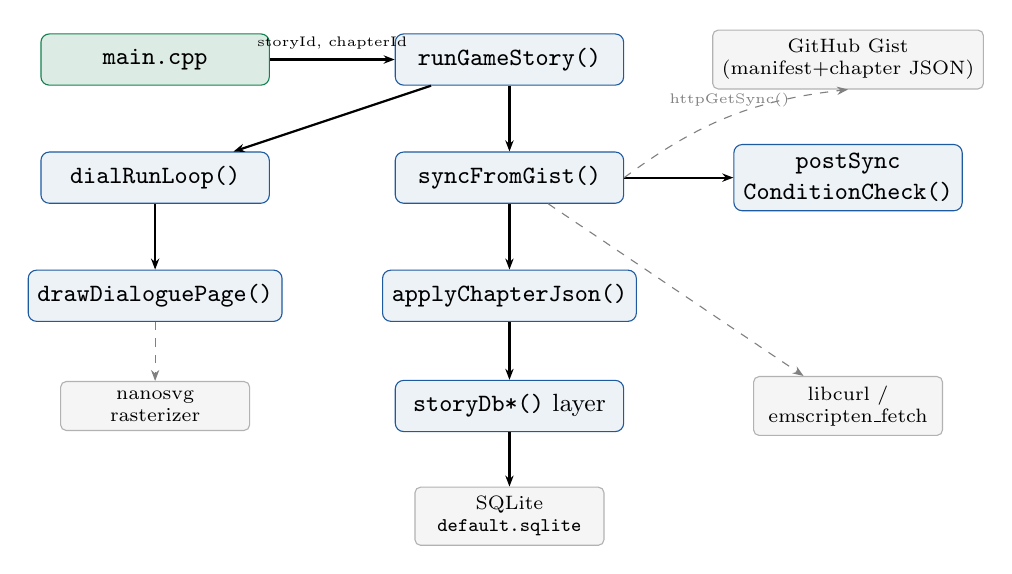
\begin{tikzpicture}[
  comp/.style={rectangle,draw=pillarBlue,fill=pillarBlue!8,rounded corners=3pt,
               minimum width=2.9cm,minimum height=0.65cm,align=center,font=\small},
  ext/.style={rectangle,draw=gray!60,fill=gray!8,rounded corners=2pt,
              minimum width=2.4cm,minimum height=0.6cm,align=center,font=\scriptsize},
  iface/.style={-{Stealth[length=4pt]},thick},
  use/.style={-{Stealth[length=4pt]},dashed,gray}
]
  \node[comp,fill=versionGreen!15,draw=versionGreen] (main) at (0,0) {\texttt{main.cpp}};
  \node[comp] (entry)  at (4.5,0)   {\texttt{runGameStory()}};
  \node[comp] (sync)   at (4.5,-1.5){\texttt{syncFromGist()}};
  \node[comp] (apply)  at (4.5,-3.0){\texttt{applyChapterJson()}};
  \node[comp] (db)     at (4.5,-4.4){\texttt{storyDb*()} layer};
  \node[comp] (psc)    at (8.8,-1.5){\texttt{postSync}\\\texttt{ConditionCheck()}};
  \node[comp] (loop)   at (0,-1.5)  {\texttt{dialRunLoop()}};
  \node[comp] (render) at (0,-3.0)  {\texttt{drawDialoguePage()}};
  \node[ext]  (gist)  at (8.8,0)    {GitHub Gist\\(manifest+chapter JSON)};
  \node[ext]  (sqlite)at (4.5,-5.8) {SQLite\\\texttt{default.sqlite}};
  \node[ext]  (svg)   at (0,-4.4)   {nanosvg\\rasterizer};
  \node[ext]  (http)  at (8.8,-4.4) {libcurl /\\emscripten\_fetch};
  \draw[iface](main)--(entry)  node[above,font=\tiny,midway]{storyId, chapterId};
  \draw[iface](entry)--(sync);
  \draw[iface](entry)--(loop);
  \draw[iface](sync)--(apply);
  \draw[iface](apply)--(db);
  \draw[iface](db)--(sqlite);
  \draw[iface](loop)--(render);
  \draw[use]  (render)--(svg);
  \draw[iface](sync)--(psc);
  \draw[use]  (sync.east)to[bend left=15]node[above,font=\tiny]{httpGetSync()}(gist.south);
  \draw[use]  (sync)--(http);
\end{tikzpicture}
\end{center}

% ----------------------------------------------------------
\subsection{Thuật toán cốt lõi}

\subsubsection{SVG Lazy-Init Rasterizer (V1)}

\begin{center}
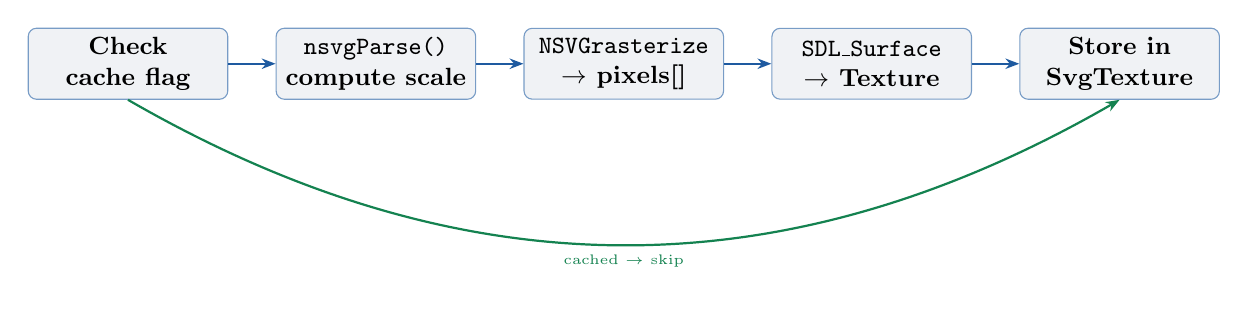
\begin{tikzpicture}[node distance=0.5cm,
  b/.style={sdsBox=pillarBlue!60,text width=2.3cm}]
  \node[b](a){Check\\cache flag};
  \node[b,right=0.6cm of a](b){\texttt{nsvgParse()}\\compute scale};
  \node[b,right=0.6cm of b](c){\texttt{NSVGrasterize}\\$\rightarrow$ pixels[]};
  \node[b,right=0.6cm of c](d){\texttt{SDL\_Surface}\\$\rightarrow$ Texture};
  \node[b,right=0.6cm of d](e){Store in\\SvgTexture};
  \foreach \x/\y in {a/b,b/c,c/d,d/e}{\draw[sdsArrow=pillarBlue](\x)--(\y);}
  \draw[sdsArrow=versionGreen,bend right=30](a.south)to
      node[below,font=\tiny]{cached $\rightarrow$ skip}(e.south);
\end{tikzpicture}
\end{center}

\noindent Công thức fade-in:
$\alpha(t) = \bigl\lfloor\min(1,\; t / T_\text{intro}) \times 255\bigr\rfloor$,
\quad $T_\text{intro} = 8000\,\text{ms}$.

Scale SVG về \texttt{targetW}: $\texttt{scale} = \texttt{targetW} / \texttt{image->width}$;
$\texttt{outH} = \lfloor \texttt{image->height} \times \texttt{scale} + 0.5 \rfloor$.

\subsubsection{Gist SHA-diff Sync --- \texttt{syncFromGist()}}

\begin{center}
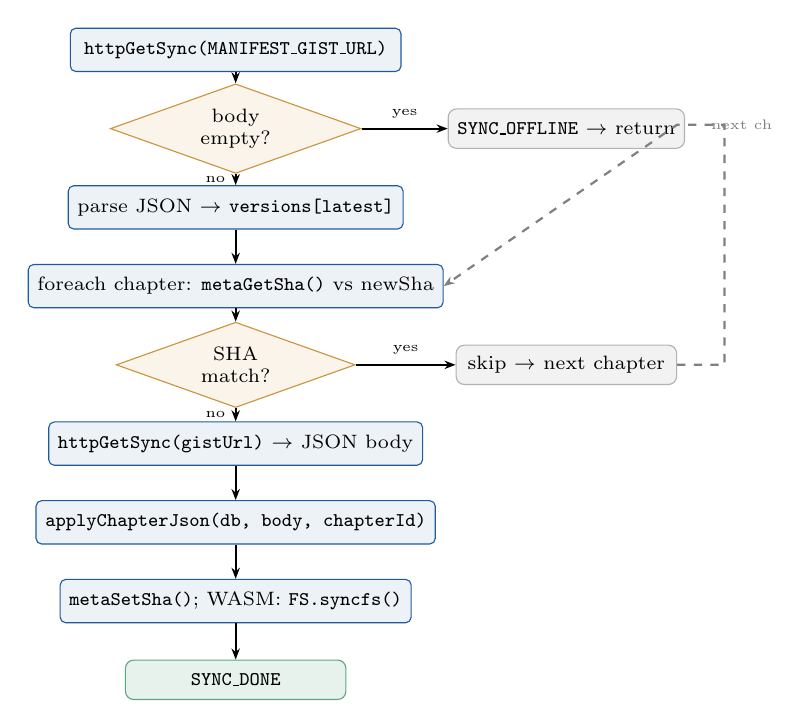
\begin{tikzpicture}[
  proc/.style={rectangle,draw=pillarBlue,fill=pillarBlue!8,rounded corners=2pt,
               minimum width=4.2cm,minimum height=0.55cm,align=center,font=\scriptsize},
  dec/.style={diamond,draw=versionAmber!80,fill=versionAmber!8,
              aspect=2.8,align=center,font=\scriptsize},
  term/.style={rectangle,rounded corners=3pt,draw=gray!60,fill=gray!10,
               minimum width=2.8cm,minimum height=0.5cm,align=center,font=\scriptsize},
  wterm/.style={rectangle,rounded corners=3pt,draw=versionGreen!70,fill=versionGreen!10,
                minimum width=2.8cm,minimum height=0.5cm,align=center,font=\scriptsize},
  arr/.style={-{Stealth[length=4pt]},thick}
]
  \node[proc](p0) at (0,0)    {\texttt{httpGetSync(MANIFEST\_GIST\_URL)}};
  \node[dec] (d0) at (0,-1.0) {body\\empty?};
  \node[term](off)at (4.2,-1.0){\texttt{SYNC\_OFFLINE} $\rightarrow$ return};
  \node[proc](p1) at (0,-2.0) {parse JSON $\rightarrow$ \texttt{versions[latest]}};
  \node[proc](p2) at (0,-3.0) {foreach chapter: \texttt{metaGetSha()} vs newSha};
  \node[dec] (d1) at (0,-4.0) {SHA\\match?};
  \node[term](sk) at (4.2,-4.0){skip $\rightarrow$ next chapter};
  \node[proc](p3) at (0,-5.0) {\texttt{httpGetSync(gistUrl)} $\rightarrow$ JSON body};
  \node[proc](p4) at (0,-6.0) {\texttt{applyChapterJson(db, body, chapterId)}};
  \node[proc](p5) at (0,-7.0) {\texttt{metaSetSha()}; WASM: \texttt{FS.syncfs()}};
  \node[wterm](dn)at (0,-8.0) {\texttt{SYNC\_DONE}};
  \draw[arr](p0)--(d0);
  \draw[arr](d0)--node[above,font=\tiny]{yes}(off);
  \draw[arr](d0)--node[left,font=\tiny]{no}(p1);
  \draw[arr](p1)--(p2); \draw[arr](p2)--(d1);
  \draw[arr](d1)--node[above,font=\tiny]{yes}(sk);
  \draw[arr](d1)--node[left,font=\tiny]{no}(p3);
  \draw[arr](p3)--(p4); \draw[arr](p4)--(p5); \draw[arr](p5)--(dn);
  % loop-back arrow for chapters
  \draw[arr,gray,dashed](sk.east)--++(0.6,0)--++(0,3.05)--
      node[right,font=\tiny]{next ch}++(-0.6,0)--(p2.east);
\end{tikzpicture}
\end{center}

\noindent\textbf{applyChapterJson()} --- một SQLite transaction per \texttt{idChapter}:
\begin{enumerate}[nosep,label=\arabic*.]
  \item Tập hợp \texttt{incomingIds[]} từ JSON;
        xác định \texttt{idChapter} từ row đầu tiên.
  \item \texttt{DELETE} \texttt{shared\_data / dialogues / choices} WHERE
        \texttt{idChapter=N AND idStory NOT IN (incomingIds)}.
  \item \texttt{BEGIN;} UPSERT từng row \texttt{shared\_data}; per story: DELETE cũ rồi
        re-INSERT \texttt{shared\_dialogues} + \texttt{shared\_choices};
        \texttt{COMMIT;}.
\end{enumerate}

\subsubsection{Dialogue State Machine --- \texttt{dialRunLoop()}}

\begin{center}
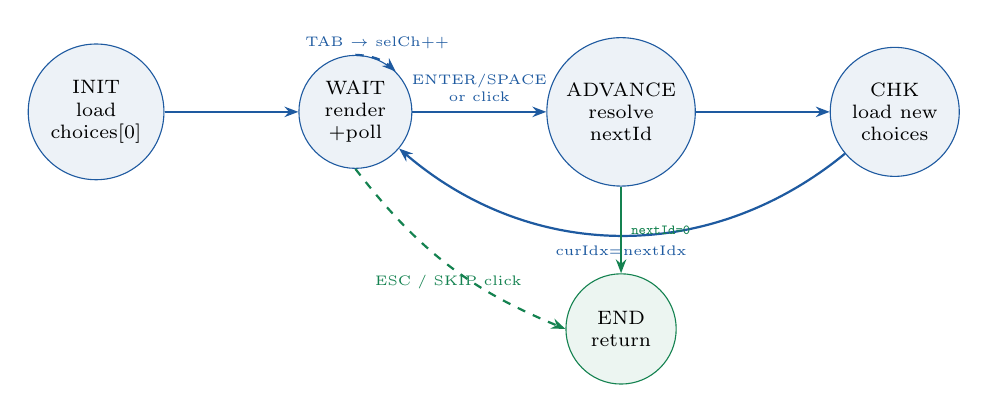
\begin{tikzpicture}[node distance=1.7cm,
  st/.style={circle,draw=pillarBlue,fill=pillarBlue!8,font=\scriptsize,
             minimum size=1.4cm,align=center}]
  \node[st](init){INIT\\load\\choices[0]};
  \node[st,right=of init](wait){WAIT\\render\\+poll};
  \node[st,right=of wait](adv) {ADVANCE\\resolve\\nextId};
  \node[st,right=of adv] (chk) {CHK\\load new\\choices};
  \node[st,below=1.1cm of adv,draw=versionGreen,fill=versionGreen!8](end){END\\return};
  \draw[sdsArrow=pillarBlue](init)--(wait);
  \draw[sdsArrow=pillarBlue](wait)--node[above, align=center, font=\tiny]{ENTER/SPACE\\or click}(adv);
  \draw[sdsArrow=pillarBlue](adv)--(chk);
  \draw[sdsArrow=pillarBlue,bend left=40](chk)to
      node[below,font=\tiny]{curIdx=nextIdx}(wait);
  \draw[sdsArrow=versionGreen](adv)--node[right,font=\tiny]{\texttt{nextId=0}}(end);
  \draw[sdsArrow=versionGreen,dashed](wait.south)to[bend right=15]
      node[below,font=\tiny]{ESC / SKIP click}(end.west);
  \draw[sdsArrow=pillarBlue,dashed](wait.north)to[bend left=20]
      node[above,font=\tiny]{TAB $\rightarrow$ selCh++}(wait.north east);
\end{tikzpicture}
\end{center}

\noindent\textbf{Word-wrap algorithm} (\texttt{diagDrawWrapped()} — max 30 chars/dòng,
12 dòng):
\begin{enumerate}[nosep,label=\arabic*.]
  \item \texttt{take = min(rem, 30)}.
  \item Nếu \texttt{take==30} và \texttt{pos+take < len}: quét ngược tìm space $\rightarrow$ điều chỉnh \texttt{take}.
  \item \texttt{SDL\_RenderDebugText()}; \texttt{y += 14.0f};
        bỏ leading spaces.
\end{enumerate}

\subsubsection{Post-sync Condition Check --- Return Value Contract}\label{sec:postSyncSRS}

\noindent\textit{State-machine diagram đã trình bày trong SRS §\ref{sec:postSyncSRS}.
SDS bổ sung implementation contract:}

\begin{center}\small
\begin{tabular}{@{}c p{4.5cm} p{5.5cm}@{}}
\hline
\textbf{Return} & \textbf{Điều kiện DB} & \textbf{Hành động trong \texttt{runGameStory}} \\
\hline
\texttt{0}  & Không có \texttt{isSelected=1};
            không có story ở chapter 1
            & Thoát $\rightarrow$ Console (không chạy dialogue) \\
\texttt{+N} & Story N là first-time hoặc replay
            & \texttt{storyDbLoadDialogue(N,ch)} $\rightarrow$ \texttt{dialRunLoop()} \\
\texttt{-N} & Story N vừa unlock (\texttt{maxScore$\geq$minScore} và
              \texttt{maxSpeed$\geq$minSpeed})
            & Hiển thị YES/NO prompt;
              YES $\rightarrow$ \texttt{UPDATE isSelected} +
              \texttt{FS.syncfs} + \texttt{dialRunLoop(N)} \\
\hline
\end{tabular}
\end{center}

% ----------------------------------------------------------
\subsection{Cấu trúc dữ liệu}

\subsubsection{C++ Runtime Structs}

\begin{verbatim}
// gameStory_db.h (public)
struct DialogueNode {
    int         nodeId;
    std::string speaker, text, imageUrl, bgmUrl, sfxUrl;
    int         nextNodeId;
    // 0 = terminal node
    bool        hasChoices;
};
struct DialogueChoice {
    int         choiceIdx;
    // 0-based display order
    std::string label;
    int         nextNodeId;
};
// app.cpp (module-internal)
struct SvgTexture   { SDL_Texture* texture = nullptr; int w = 0, h = 0; };
enum   SyncState    { SYNC_IDLE, SYNC_FETCHING, SYNC_UPDATING_DB,
                      SYNC_DONE, SYNC_OFFLINE };
struct SyncProgress { int total = 0, done = 0;
                      std::string currentId; SyncState state = SYNC_IDLE; };
\end{verbatim}

\subsubsection{SQLite ERD}

\begin{center}
\newcommand{\pk}[1]{\underline{#1}}
\begin{tikzpicture}[
  ent/.style={rectangle,draw=pillarBlue,fill=pillarBlue!6,rounded corners=2pt,
              align=left,font=\scriptsize,inner sep=5pt,minimum width=3.4cm},
  rw/.style={rectangle,draw=versionGreen,fill=versionGreen!6,rounded corners=2pt,
             align=left,font=\scriptsize,inner sep=5pt,minimum width=3.4cm},
  rel/.style={-{Stealth[length=4pt]},thick,pillarBlue!70},
  wrrel/.style={-{Stealth[length=4pt]},thick,versionGreen!80},
  lbl/.style={font=\tiny,fill=white,inner sep=1pt}
]
  \node[ent](sd) at (0,0) {
    \textbf{shared\_data}\ \textit{\tiny(R-only)}\\[1pt]
    \pk{idStory, idChapter}\\
    storyName, chapterName\\
    minScore, minSpeed, minRetries\\
    requiredStories, thumbnailPath
  };
  \node[ent](dlg) at (7,1.4) {
    \textbf{shared\_dialogues}\ \textit{\tiny(R-only)}\\[1pt]
    \pk{idStory, idChapter, nodeId}\\
    speaker, text\\
    imageUrl, bgmUrl, sfxUrl\\
    nextNodeId, hasChoices
  };
  \node[ent](cho) at (7,-1.8) {
    \textbf{shared\_choices}\ \textit{\tiny(R-only)}\\[1pt]
    \pk{idStory, idChapter,}\\
    \pk{nodeId, choiceIdx}\\
    label, nextNodeId
  };
  \node[rw](meta) at (0,-3.6) {
    \textbf{shared\_meta}\ \textit{\tiny(R/W $\leftarrow$ gameStory)}\\[1pt]
    \pk{chapter\_id} \textit{\tiny(e.g. ''c001'')}\\
    sha, updated\_at\\
    media\_base\_url
  };
  \node[rw](us) at (7,-3.8) {
    \textbf{idUser\_Stories}\ \textit{\tiny(R/W $\leftarrow$ gameStory)}\\[1pt]
    \pk{idUser, idStory, idChapter}\\
    isActivated, isSelected\\
    lastMaxScore, lastMaxSpeed
  };
  % shared_data $\rightarrow$ shared_dialogues (1:N on idStory+idChapter)
  \draw[rel](sd.north east)to[bend left=10]
      node[lbl,pos=0.3]{1}node[lbl,pos=0.75]{N}(dlg.west);
  % shared_dialogues $\rightarrow$ shared_choices (1:N on idStory+idChapter+nodeId)
  \draw[rel](dlg.south)--node[lbl,left,pos=0.4]{1}node[lbl,pos=0.85]{N}(cho.north);
  % shared_data $\rightarrow$ shared_choices direct FK (idStory+idChapter)
  \draw[rel](sd.east)to[bend right=8]
      node[lbl,below,pos=0.3]{1}node[lbl,pos=0.78]{N}(cho.west);
  % shared_meta linked to shared_data by chapter scope (dashed, logical)
  \draw[wrrel,dashed](meta.east)--
      node[lbl,above,pos=0.45]{chapter\_id ↔ idChapter (logical)}(sd.south);
  % shared_data $\rightarrow$ idUser_Stories
  \draw[wrrel](sd.east)to[bend left=8]
      node[lbl,pos=0.3]{1}node[lbl,pos=0.78]{0..1/user}(us.west);
\end{tikzpicture}
\end{center}

\subsubsection{Dataflow Diagram --- Intro Path (\texttt{storyId=0})}

\begin{center}
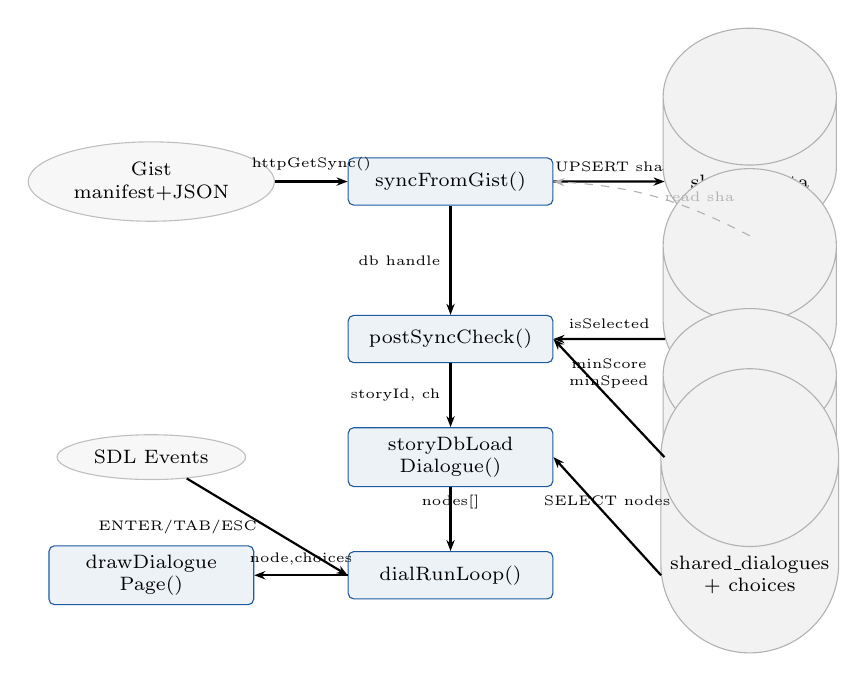
\begin{tikzpicture}[
  proc/.style={rectangle,draw=pillarBlue,fill=pillarBlue!8,rounded corners=2pt,
               minimum width=2.6cm,minimum height=0.6cm,align=center,font=\scriptsize},
  store/.style={cylinder,draw=gray!60,fill=gray!10,shape border rotate=90,
                minimum width=2.2cm,minimum height=0.55cm,align=center,font=\scriptsize},
  extio/.style={ellipse,draw=gray!50,fill=gray!6,minimum width=1.8cm,
                minimum height=0.5cm,align=center,font=\scriptsize},
  fl/.style={-{Stealth[length=4pt]},thick},
  dfl/.style={-{Stealth[length=4pt]},dashed,gray!60}
]
  \node[extio](gist) at (0,5)    {Gist\\manifest+JSON};
  \node[proc] (sync) at (3.8,5)  {syncFromGist()};
  \node[store](meta) at (7.6,5)  {shared\_meta};
  \node[proc] (psc)  at (3.8,3)  {postSyncCheck()};
  \node[store](us)   at (7.6,3)  {idUser\_Stories};
  \node[store](sdat) at (7.6,1.5){shared\_data};
  \node[proc] (load) at (3.8,1.5){storyDbLoad\\Dialogue()};
  \node[store](sdlg) at (7.6,0)  {shared\_dialogues\\+ choices};
  \node[proc] (loop) at (3.8,0)  {dialRunLoop()};
  \node[proc] (draw) at (0,0)    {drawDialogue\\Page()};
  \node[extio](user) at (0,1.5)  {SDL Events};
  \draw[fl](gist)--node[above,font=\tiny]{httpGetSync()}(sync);
  \draw[fl](sync)--node[above,font=\tiny]{UPSERT sha}(meta);
  \draw[dfl](meta.south)to[bend right=12]
      node[right,font=\tiny]{read sha}(sync.east);
  \draw[fl](sync)--node[left,font=\tiny]{db handle}(psc);
  \draw[fl](us.west)--node[above,font=\tiny]{isSelected}(psc.east);
  \draw[fl](sdat.west)--node[above, align=center, font=\tiny]{minScore\\minSpeed}(psc.east);
  \draw[fl](psc)--node[left,font=\tiny]{storyId, ch}(load);
  \draw[fl](sdlg.west)--node[above,font=\tiny]{SELECT nodes}(load.east);
  \draw[fl](load)--node[above,font=\tiny]{nodes[]}(loop);
  \draw[fl](loop)--node[above,font=\tiny]{node,choices}(draw);
  \draw[fl](user)--node[left,font=\tiny]{ENTER/TAB/ESC}(loop.west);
\end{tikzpicture}
\end{center}

\subsubsection{Sequence Diagram --- Hai Entry Path}

\begin{center}
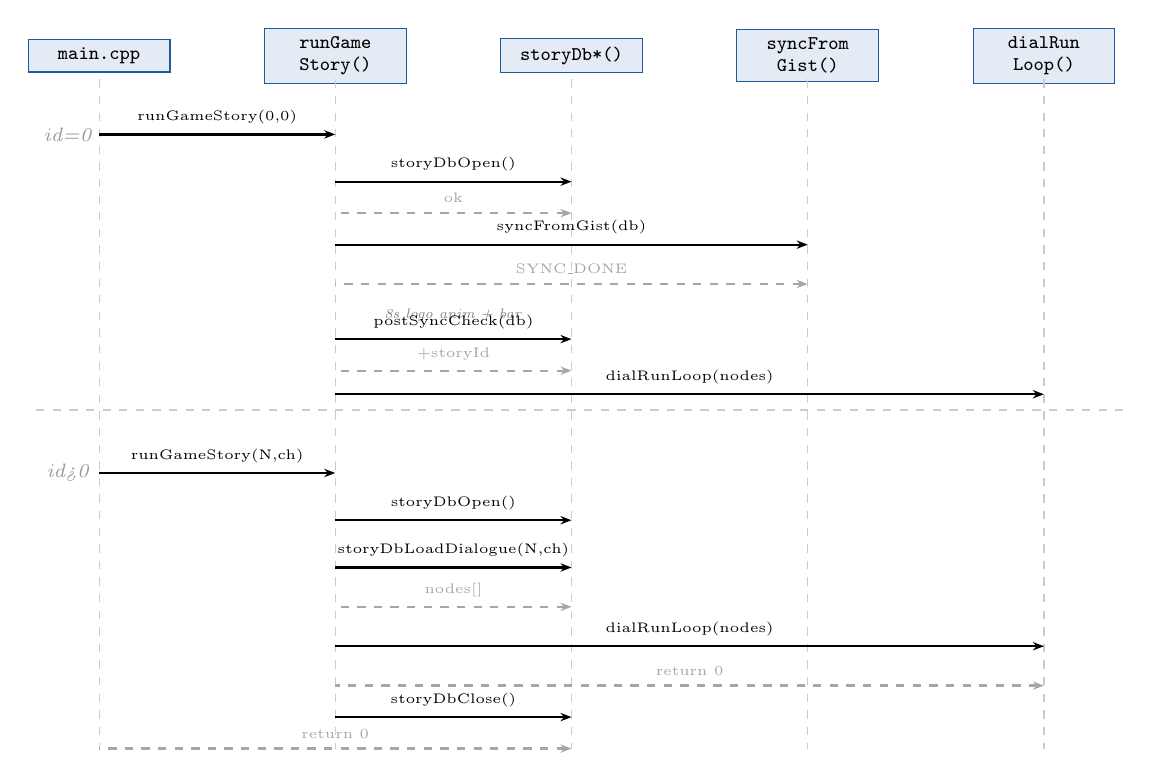
\begin{tikzpicture}[
  lhd/.style={rectangle,fill=pillarBlue!12,draw=pillarBlue,font=\scriptsize,
              inner sep=3pt,minimum width=1.8cm,align=center},
  msg/.style={-{Stealth[length=4pt]},thick},
  ret/.style={{Stealth[length=4pt]}-,thick,dashed,gray!70},
  lf/.style={draw=gray!40,dashed}
]
  % headers
  \node[lhd] (H1) at (0,0)    {\texttt{main.cpp}};
  \node[lhd] (H2) at (3.0,0)  {\texttt{runGame}\\\texttt{Story()}};
  \node[lhd] (H3) at (6.0,0)  {\texttt{storyDb*()}};
  \node[lhd] (H4) at (9.0,0)  {\texttt{syncFrom}\\\texttt{Gist()}};
  \node[lhd] (H5) at (12.0,0) {\texttt{dialRun}\\\texttt{Loop()}};
  % lifelines
  \foreach \x in {0,3.0,6.0,9.0,12.0} { \draw[lf](\x,-0.3)--(\x,-8.8); }
  % ---- path label divider
  \draw[gray!40,thick,dashed](-0.8,-4.5)--(13,-4.5);
  \node[font=\scriptsize\itshape,gray!80] at (-0.4,-1.0) {id=0};
  \node[font=\scriptsize\itshape,gray!80] at (-0.4,-5.3) {id>0};
  % ---- storyId=0 ----
  \draw[msg](0,-1.0)--(3.0,-1.0)   node[above,font=\tiny,midway]{runGameStory(0,0)};
  \draw[msg](3.0,-1.6)--(6.0,-1.6) node[above,font=\tiny,midway]{storyDbOpen()};
  \draw[ret](6.0,-2.0)--(3.0,-2.0) node[above,font=\tiny,midway]{ok};
  \draw[msg](3.0,-2.4)--(9.0,-2.4) node[above,font=\tiny,midway]{syncFromGist(db)};
  \draw[ret](9.0,-2.9)--(3.0,-2.9) node[above,font=\tiny,midway]{SYNC\_DONE};
  \node[font=\tiny,gray] at (4.5,-3.3) {\textit{8s logo anim + bar}};
  \draw[msg](3.0,-3.6)--(6.0,-3.6) node[above,font=\tiny,midway]{postSyncCheck(db)};
  \draw[ret](6.0,-4.0)--(3.0,-4.0) node[above,font=\tiny,midway]{+storyId};
  \draw[msg](3.0,-4.3)--(12.0,-4.3)node[above,font=\tiny,midway]{dialRunLoop(nodes)};
  % ---- storyId>0 ----
  \draw[msg](0,-5.3)--(3.0,-5.3)   node[above,font=\tiny,midway]{runGameStory(N,ch)};
  \draw[msg](3.0,-5.9)--(6.0,-5.9) node[above,font=\tiny,midway]{storyDbOpen()};
  \draw[msg](3.0,-6.5)--(6.0,-6.5) node[above,font=\tiny,midway]{storyDbLoadDialogue(N,ch)};
  \draw[ret](6.0,-7.0)--(3.0,-7.0) node[above,font=\tiny,midway]{nodes[]};
  \draw[msg](3.0,-7.5)--(12.0,-7.5)node[above,font=\tiny,midway]{dialRunLoop(nodes)};
  \draw[ret](12.0,-8.0)--(3.0,-8.0)node[above,font=\tiny,midway]{return 0};
  \draw[msg](3.0,-8.4)--(6.0,-8.4) node[above,font=\tiny,midway]{storyDbClose()};
  \draw[ret](6.0,-8.8)--(0,-8.8)   node[above,font=\tiny,midway]{return 0};
\end{tikzpicture}
\end{center}

% ----------------------------------------------------------
\subsection{Giao diện công khai}

\begin{verbatim}
// extern declared in app/main.cpp
int runGameStory(SDL_Window* window,
                 SDL_Renderer* renderer,
                 int storyId   = 0,
                 int chapterId = 0);

// Returns: always 0.  Caller does NOT branch on return value.

// gameStory_db.h — module-internal, not linked by gameConsole/gameCore
bool                        storyDbOpen();
void                        storyDbClose();

std::vector<DialogueNode>   storyDbLoadDialogue(int idStory, int idChapter);
std::vector<DialogueChoice> storyDbLoadChoices (int idStory, int idChapter,
                                                 int nodeId);

\end{verbatim}

\noindent\textbf{Compile-time define} (inject via \texttt{app/.env}):
\begin{verbatim}
-DMANIFEST_GIST_URL="https://gist.githubusercontent.com/..."
// Empty string $\rightarrow$ auto SYNC_OFFLINE fallback, no crash.

\end{verbatim}

% ----------------------------------------------------------
\subsection{Thư viện phụ thuộc}

\begin{tabularx}{\linewidth}{@{}l l X@{}}
\hline
\textbf{Thư viện} & \textbf{Guard} & \textbf{Vai trò} \\
\hline
SDL3 / SDL3\_ttf    & always       & Window, renderer, events, \texttt{SDL\_RenderDebugText} \\
sqlite3             & always       & R/W \texttt{default.sqlite} \\
nanosvg             & always       & SVG parse;
single-header; impl compiled once in \texttt{nanosvg\_impl.cpp} \\
nanosvgrast         & always       & SVG rasterize \\
nlohmann/json       & always       & Manifest + chapter JSON parse \\
libcurl             & \texttt{\#ifdef HAVE\_LIBCURL} (native) & Blocking HTTP GET;
\texttt{-lcurl} at link \\
emscripten\_fetch   & \texttt{\#ifdef \_\_EMSCRIPTEN\_\_}     & Async-capable HTTP GET;
requires \texttt{-sASYNCIFY=1} \\
\hline
\end{tabularx}

% ═══════════════════════════════════════════════════════
\PartVersions
% ═══════════════════════════════════════════════════════

\begin{VersionTable}
\Vone & Logo animation, brand identity, BUILD\_STANDALONE
      & SDL3, nanosvg/rast
      & Standalone $\rightarrow$ \texttt{runGameStory(win,ren)} entry \\
\Vtwo & Dialogue engine, Gist SHA-diff sync, post-sync condition check
      & sqlite3, nlohmann/json, libcurl / emscripten\_fetch
      & Reads gameConsole DB;
writes \texttt{shared\_meta}, \texttt{idUser\_Stories} \\
\Vthree & Per-file media disk cache, download-speed loading bar, Atlas migration
        & emscripten\_fetch, IDBFS, Cloudflare D1
        & V3 replaces Gist $\rightarrow$ Cloudflare D1 / Durable Objects \\
\end{VersionTable}

% ----------------------------------------------------------
\subsection{\Vone\ --- Intro Animation Engine}

\textbf{Mục tiêu:} Brand identity 8\,s;
SVG lazy-init; \texttt{BUILD\_STANDALONE} mode.

\noindent\textbf{Screen layout pixel map (270×480):}

\begin{center}
\begin{tikzpicture}[x=0.72pt, y=0.72pt, every node/.style={font=\tiny}]
  \draw[thick](0,0) rectangle (270,480);
  % skip button top-right  y=5..23  (y axis inverted for display)
  \fill[gray!25](200,457) rectangle (265,475);
  \draw(200,457) rectangle (265,475);
  \node at (232,466){\texttt{SKIP\_BTN} \{200,5,65,18\}};
  % logo area  centre-ish
  \fill[pillarBlue!18](65,245) rectangle (205,355);
  \draw[pillarBlue](65,245) rectangle (205,355);
  \node[align=center] at (135,320){\texttt{LOGO\_SVG}\\targetW=140\\centre−60};
  \node at (135,300){\texttt{C T E T R I S} (grey 220,220,220)};
  % loading bar  barY = 480−110 = 370
  \fill[versionGreen!35](45,100) rectangle (225,113);
  \draw(45,100) rectangle (225,113); \node[right] at (227,107){180×12 px};
  \node[left] at (43,107){y=370};
  % status line above bar
  \draw[gray!40,dashed](45,120)--(225,120);
  \node at (135,128){\texttt{SyncState} status (y=352)};
  % corp credit below bar
  \node[align=center] at (135,80){"Powered up by " + CORP\_SVG (h=16)\\\textit{centred}};
  % axis labels
  \node[gray] at (255,470){y=0};
  \node[gray] at (255,10){y=480};
\end{tikzpicture}
\end{center}

\noindent\textbf{I/O validation:}
\begin{itemize}[nosep]
  \item $t=0$: $\alpha=0$ (transparent); $t=4000\,\text{ms}$: $\alpha=127$;
$t=8000\,\text{ms}$: $\alpha=255$.
  \item \texttt{g\_logo.texture} $\neq$ \texttt{nullptr} after first \texttt{drawLogo()} call.
  \item \texttt{runGameStory(win, ren, 0, 0)} returns \texttt{0} after $\geq8000\,\text{ms}$.

\end{itemize}

% ----------------------------------------------------------
\subsection{\Vtwo\ --- Dialogue Engine + Gist Sync}

\textbf{Mục tiêu:} Dual-mode entry; SHA-diff sync; full dialogue state machine;
post-sync condition check.

\noindent\textbf{Progress bar blending formula:}
\[
  P_{\text{bar}} = \max\!\Bigl(\underbrace{\tfrac{\texttt{done}}{\texttt{total}}}_{\text{sync}},\;
                               \underbrace{\tfrac{t}{8000}}_{\text{time}}\Bigr)
  \quad \text{(clamped to } [0,1]\text{)}
\]
\texttt{total=0} (all SHA match) $\Rightarrow$ $P_\text{sync}=1.0$ instantly.

\noindent\textbf{Choice rect layout}
(\texttt{diagChoiceRect(i, total)} — stacked from bottom of text-box):
\[
  y_i = \texttt{DIAG\_HINT\_Y} - \texttt{total}\cdot(h+g) + i\cdot(h+g),
  \quad h=22\,\text{px},\;
  g=4\,\text{px}
\]

\noindent\textbf{I/O validation:}
\begin{itemize}[nosep]
  \item SHA match $\rightarrow$ \texttt{syncProgress=1.0}; bar \texttt{fill=1.0} immediately.
  \item \texttt{storyId=1}: \texttt{storyDbLoadDialogue(1,1).size()} $\geq 1$;

  TAB increments \texttt{selCh} modulo \texttt{choices.size()}.
  \item \texttt{nextNodeId=0} on last node $\rightarrow$ \texttt{dialRunLoop()} exits;
        \texttt{runGameStory} returns \texttt{0} within one frame.

  \item \foreignlanguage{english}{\texttt{MANIFEST\_GIST\_URL=""}} $\rightarrow$ \texttt{SYNC\_OFFLINE}; no crash;
        dialogue proceeds from local DB.

\end{itemize}

% ----------------------------------------------------------
\subsection{\Vthree\ --- Media Cache + Download-speed Bar}

\textbf{Mục tiêu:} Per-file disk cache; loading bar reflects actual download speed;

logo fade-in loops until all files ready.

\noindent\textbf{Cache key:}
\foreignlanguage{english}{\texttt{SDL\_GetPrefPath("uit","cTetris") + "cache/" + \textit{basename}(url)}}.
Skip if file exists on disk.

\noindent\textbf{Download-speed bar:}
\begin{align*}
  \text{speed}_{500\text{ms}} &= \Delta\texttt{bytesDone} / 0.5\;\text{KB/s} \\
  P_\text{bar}                &= \texttt{bytesDone} / \texttt{bytesTotal}
\end{align*}
Logo fade-in cycle repeats (\texttt{elapsedTime mod } $T_\text{intro}$)
while \texttt{bytesDone} $<$ \texttt{bytesTotal}.

\noindent\textbf{URL substitution} (post-cache, no DB write):
after \texttt{storyDbLoadDialogue()} returns \texttt{nodes[]},
rewrite \texttt{DialogueNode.imageUrl} from raw GitHub URL $\rightarrow$ local cache path.

\noindent\textbf{I/O validation:}
\begin{itemize}[nosep]
  \item Clear cache dir $\rightarrow$ run $\rightarrow$ \texttt{cache/} contains exactly $N$ files
        ($N$ = distinct \texttt{imageUrl} count across loaded nodes).

  \item Re-run $\rightarrow$ zero new HTTP requests (all cache-hit).
  \item Offline: \texttt{imageUrl} not substituted $\rightarrow$ \texttt{drawDialoguePage()}
        renders grey placeholder \texttt{\{80,80,80,255\}};

  no exception thrown.
\end{itemize}

\label{LastPageGameStoryEngineering}
\end{document}